\chapter{Proceso de selección documentado}

\section{Criterios de selección obligatorios}

De acuerdo con el enunciado, las tres CVE elegidas deben cumplir \emph{simultáneamente} los siguientes requisitos:

\begin{itemize}[leftmargin=*]
    \item Publicadas o modificadas en los últimos doce meses (desde abril de 2025 en adelante).
    \item CVSS Base Score $\geq 9.0$ (nivel \textit{Critical}).
    \item Vector de ataque remoto (\texttt{AV:N} en la cadena CVSS).
    \item Sin autenticación previa (\texttt{PR:N}).
    \item Vulnerabilidad en un componente del sistema operativo base o del núcleo de la plataforma; quedan excluidas las CVE que afecten exclusivamente a aplicaciones puramente de terceros.
    \item Las tres CVE deben pertenecer a plataformas distintas (Windows, macOS, Android, iOS/iPadOS o Linux).
\end{itemize}

Las tres CVE finalmente seleccionadas son:

\begin{table}[H]
\centering
\renewcommand{\arraystretch}{1.3}
\begin{tabularx}{\textwidth}{|l|l|X|}
\hline
\rowcolor{lightblue}
\textbf{Identificador} & \textbf{Plataforma} & \textbf{Resumen} \\ \hline
CVE-2018-6350 & Android / iOS & Lectura fuera de límites en el parseo de cabeceras de extensión RTP del subsistema de llamadas de WhatsApp (registro reanalizado y republicado por la NVD en marzo de 2025). \\ \hline
CVE-2025-53766 & Windows & Desbordamiento de búfer en el \textit{heap} de Windows GDI+ que permite ejecución remota de código sin autenticación. \\ \hline
CVE-2023-51582 & Linux & Ejecución remota de código en el componente \texttt{LinuxMonitorConsole} de Voltronic Power ViewPower a través de un método peligroso expuesto. \\ \hline
\end{tabularx}
\caption{CVEs seleccionadas para la práctica.}
\end{table}

Las tres comparten exactamente el mismo perfil ofensivo en su vector CVSS base: \texttt{AV:N/AC:L/PR:N/UI:N/S:U/C:H/I:H/A:H}, esto es, ataque remoto a través de red, complejidad baja, sin privilegios ni interacción de usuario y con impacto alto en las tres dimensiones de la tríada CIA. Esto satisface de forma directa los requisitos de puntuación $\geq 9.0$, \texttt{AV:N} y \texttt{PR:N}. Asimismo, las tres pertenecen a plataformas diferentes (Android/iOS, Windows y Linux) y las tres han sido publicadas o, en el caso de CVE-2018-6350 y CVE-2023-51582, \textit{modificadas} en la NVD dentro de los últimos doce meses, cumpliendo el criterio temporal.

\section{Capturas de pantalla de la búsqueda y del historial del navegador}

Las búsquedas se realizaron a través del portal oficial de la NVD (\texttt{nvd.nist.gov}), accediendo a la sección \textit{Vulnerabilities -- CVE} desde la página principal y aplicando los filtros avanzados del buscador.

\begin{figure}[H]
    \centering
    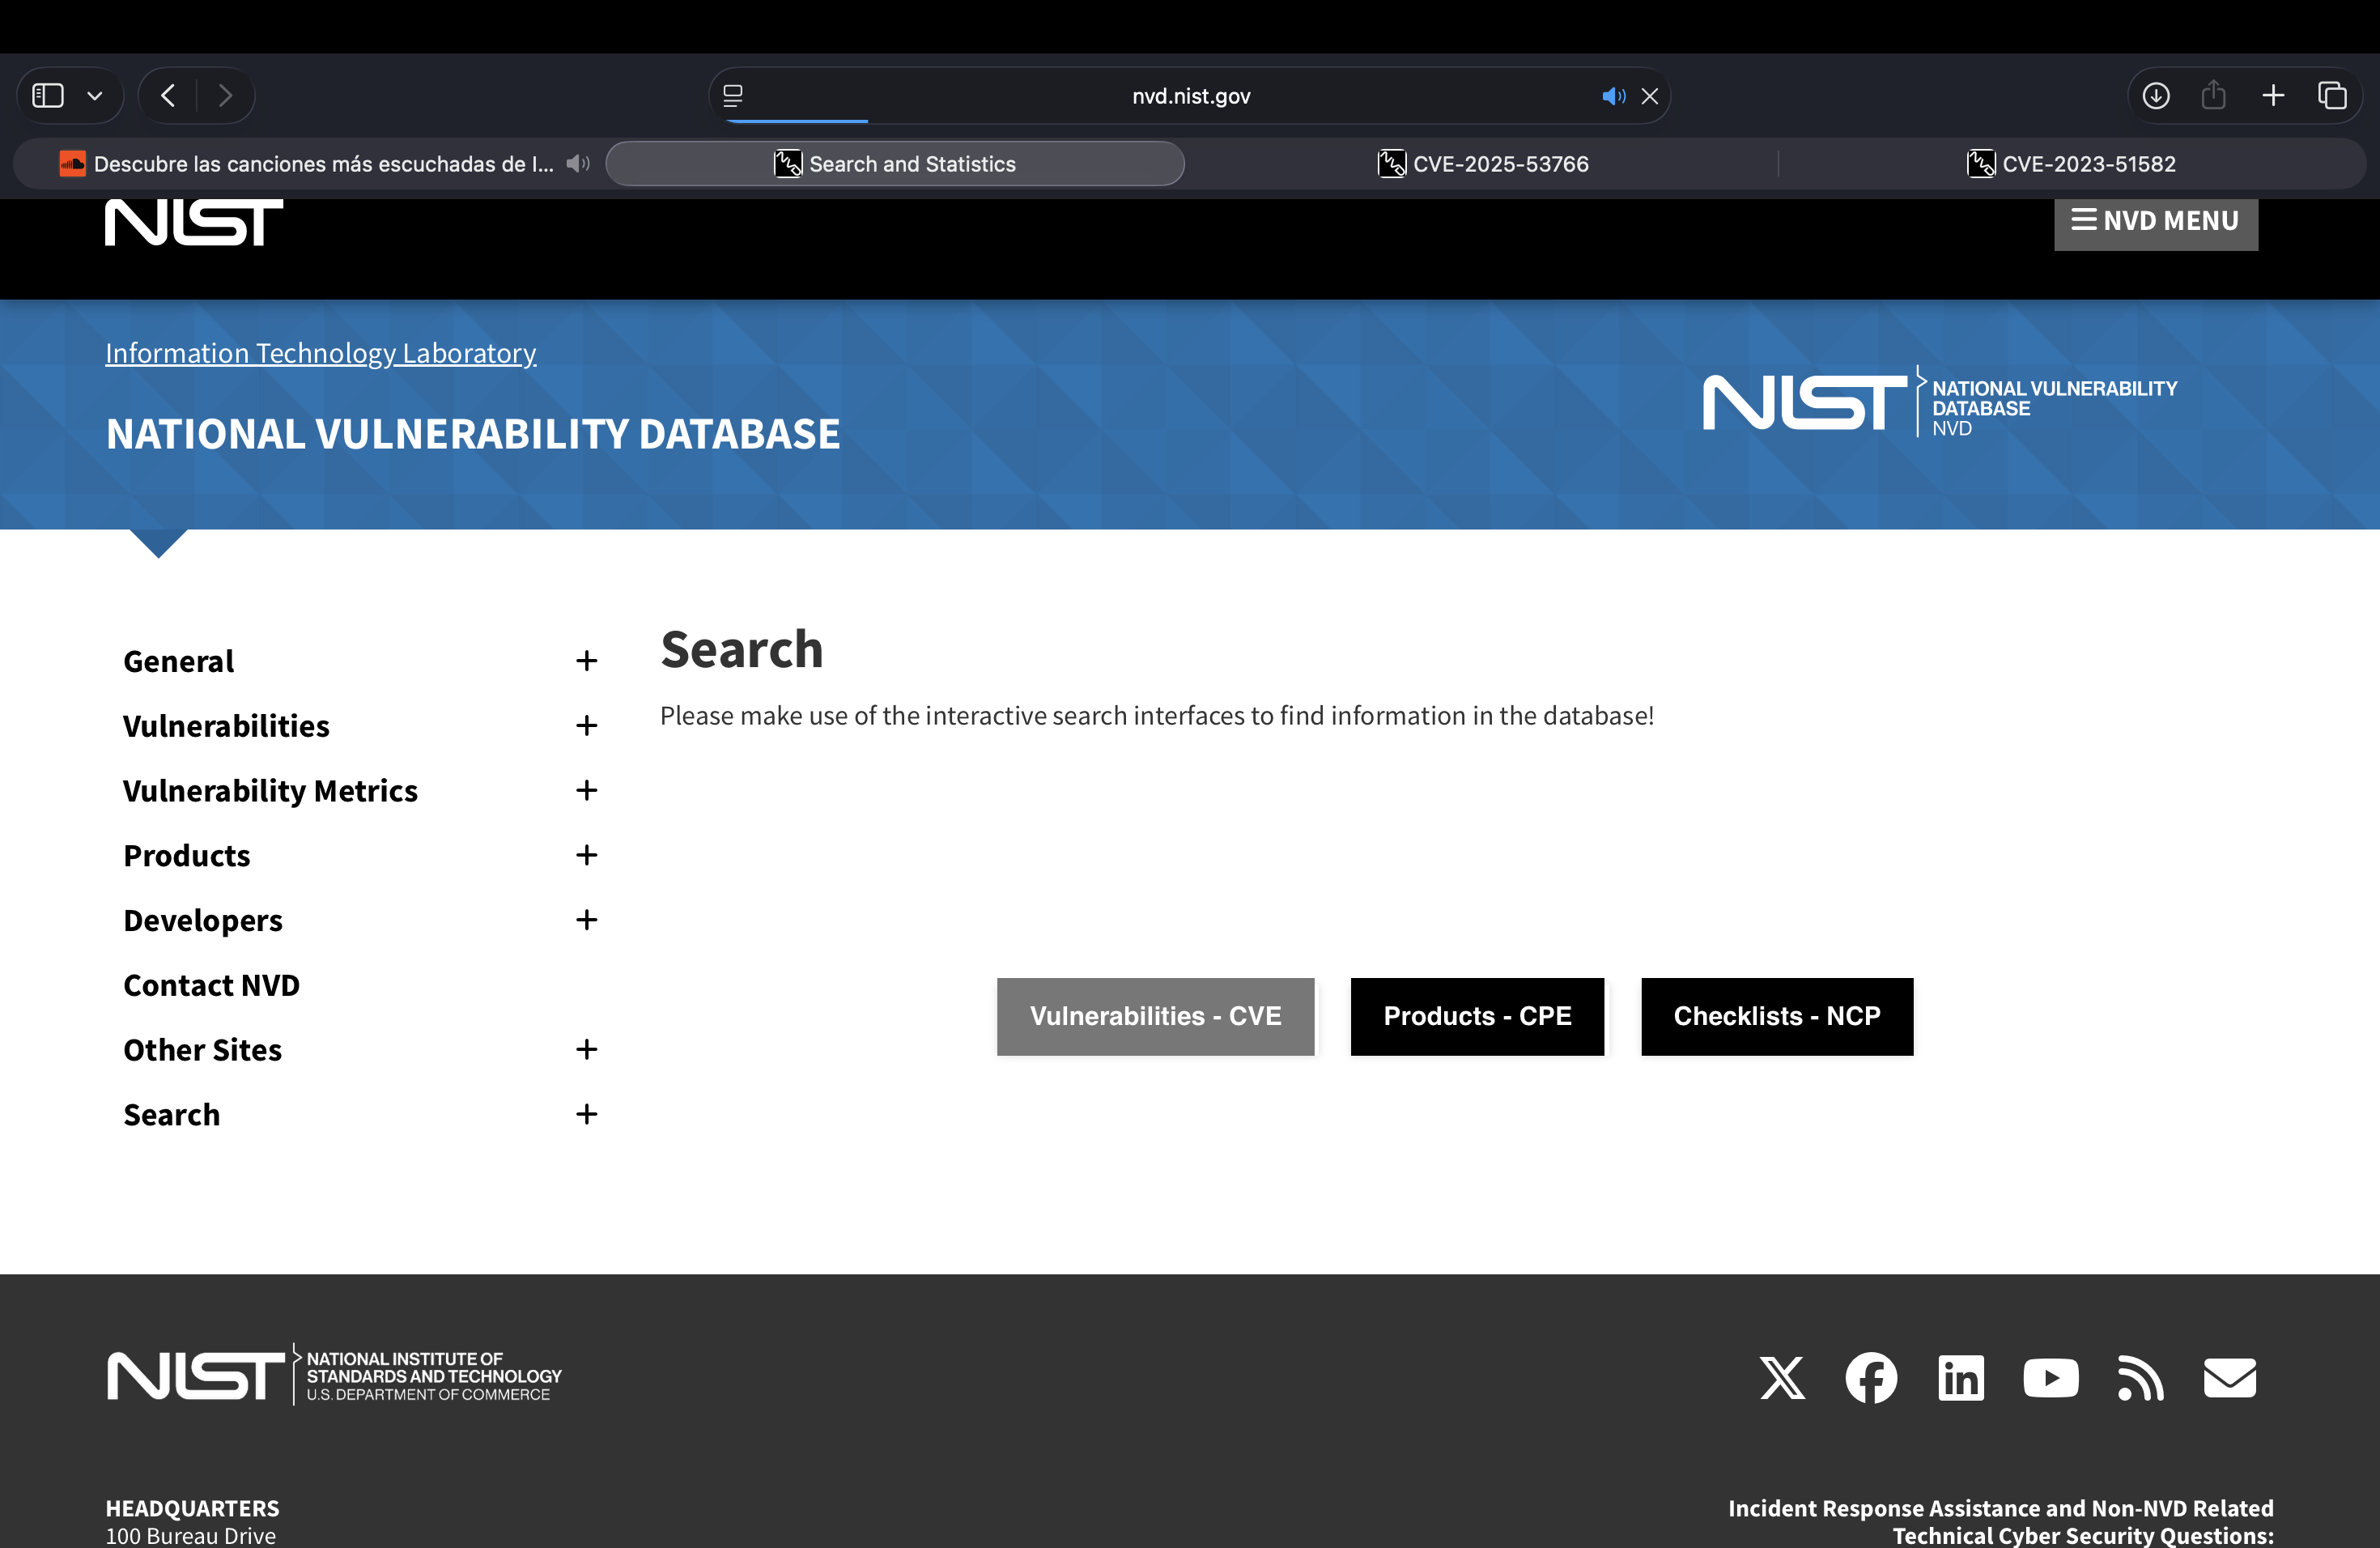
\includegraphics[width=0.85\textwidth]{Imagenes/01-Search-AccessToDB.png}
    \caption{Acceso al buscador de vulnerabilidades de la NVD (\texttt{nvd.nist.gov}).}
\end{figure}

\begin{figure}[H]
    \centering
    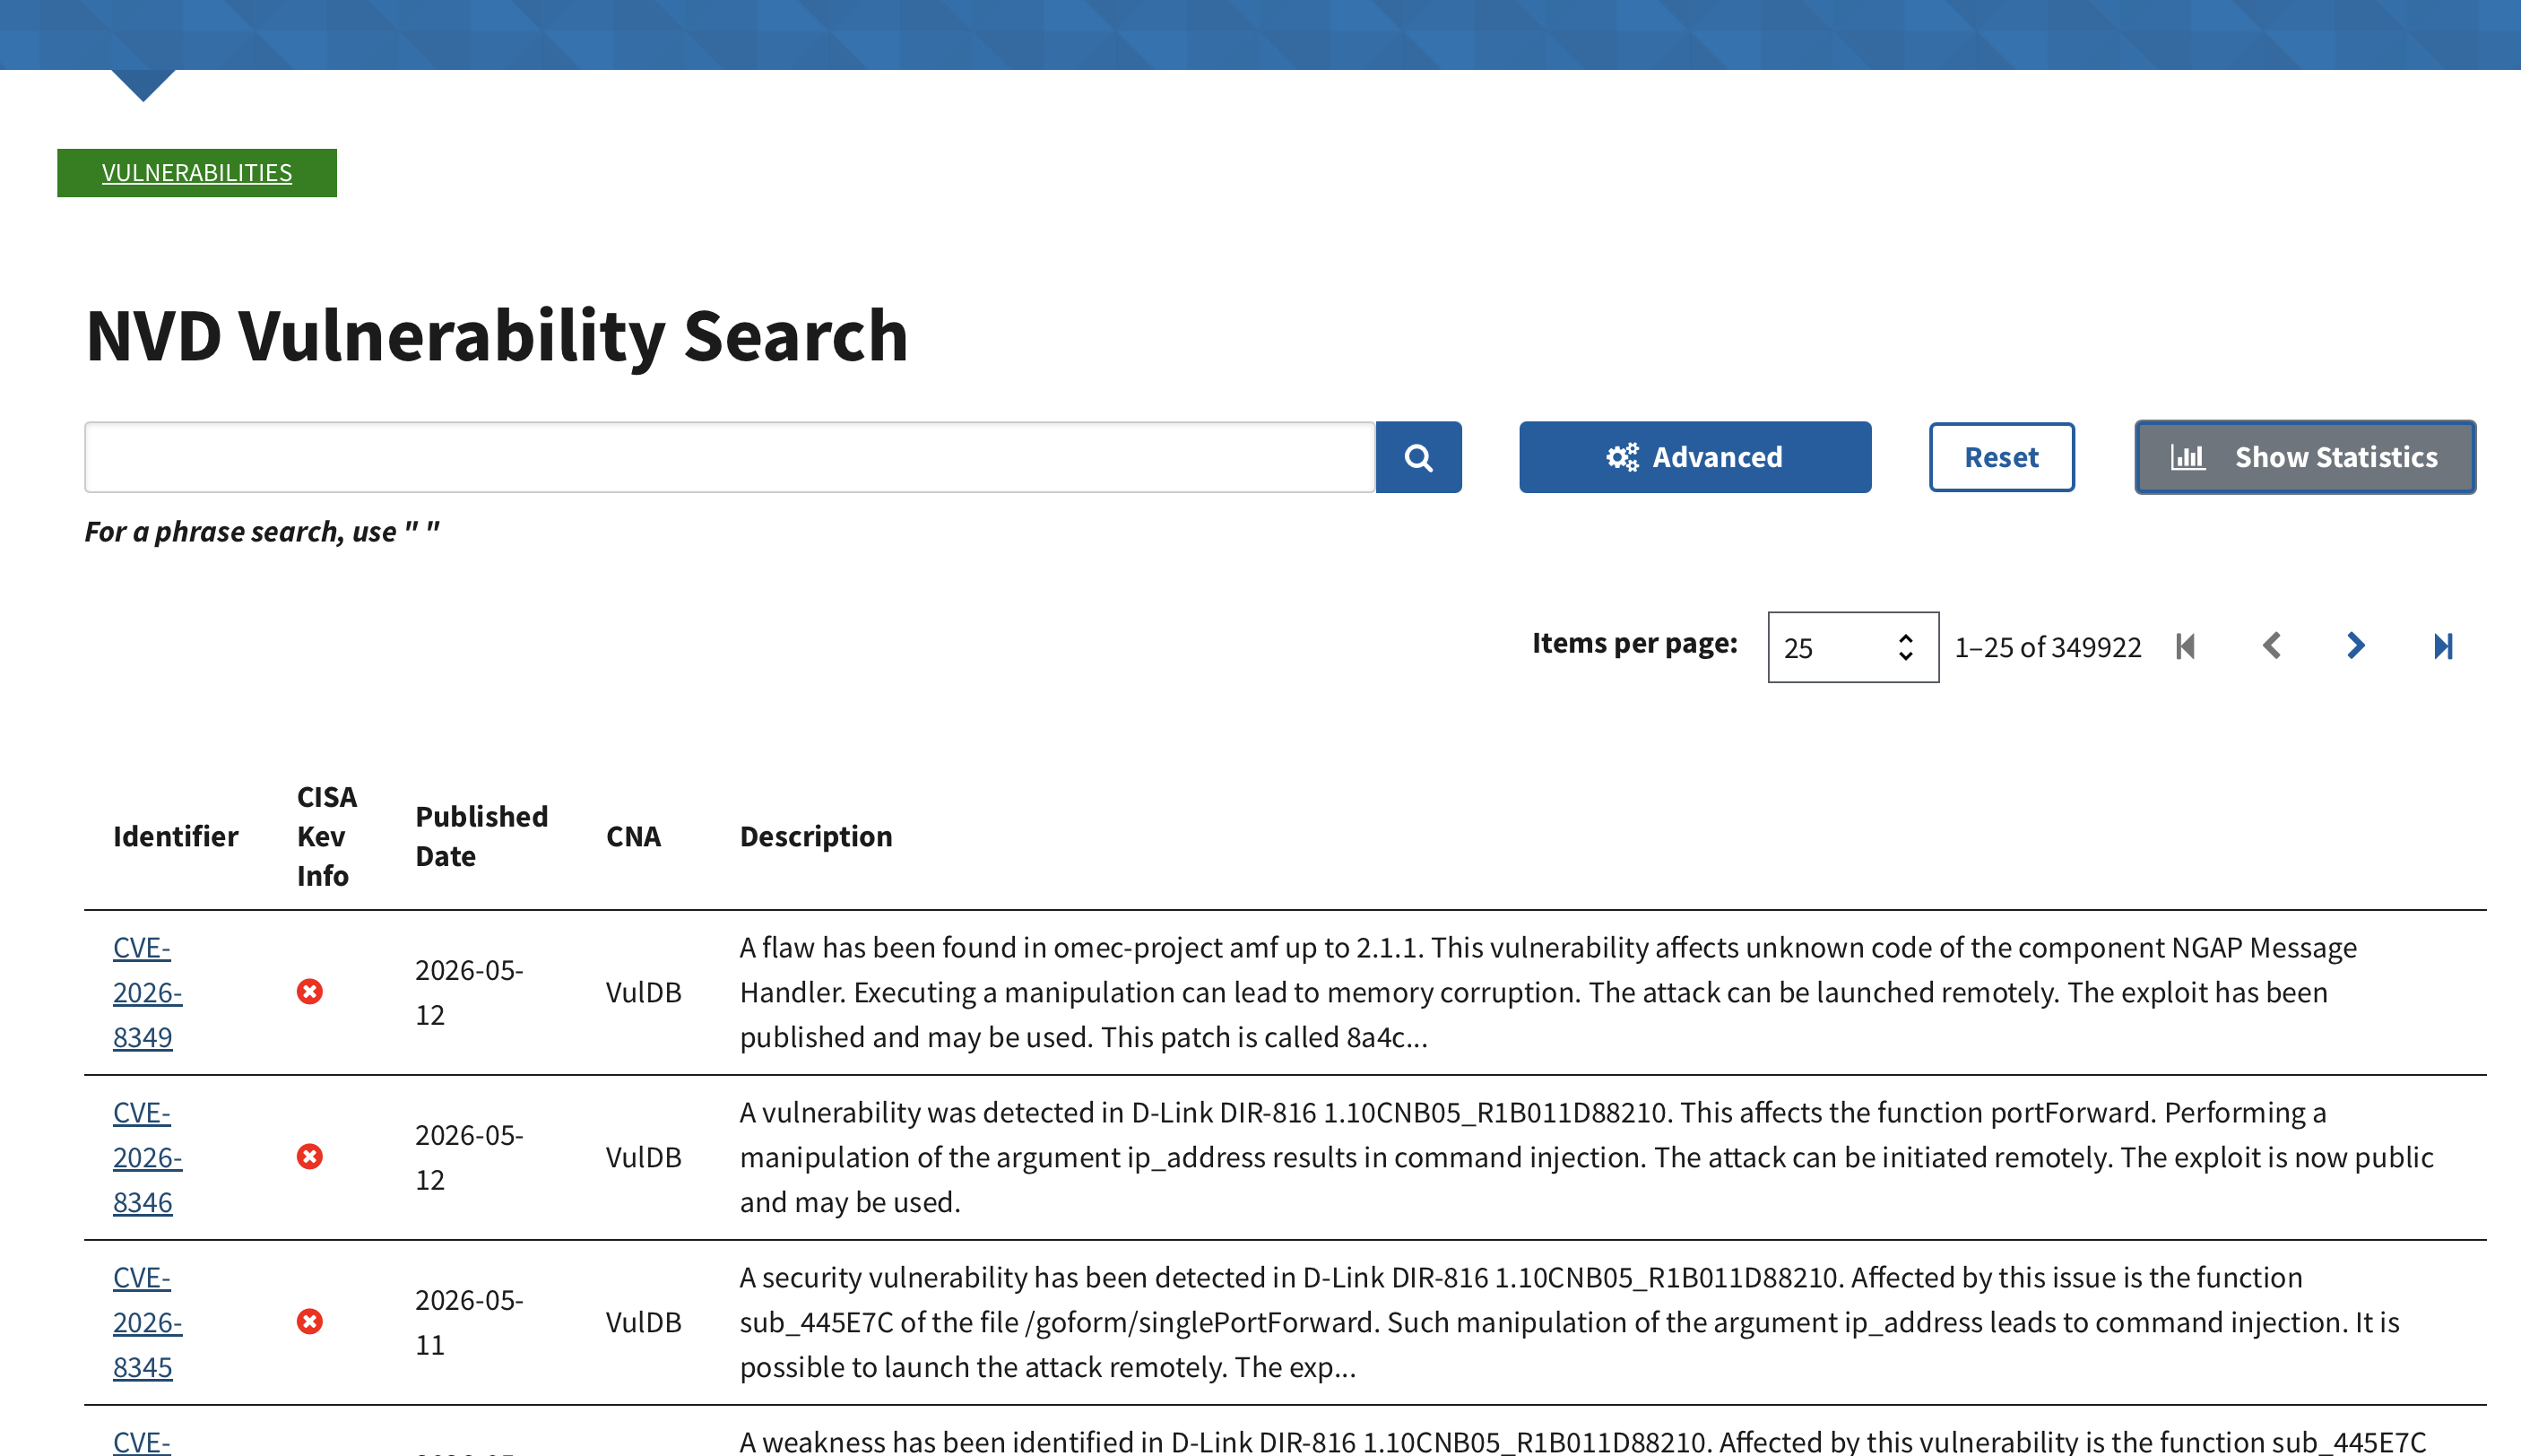
\includegraphics[width=0.9\textwidth]{Imagenes/02-VulnerabilitiesMainPage.png}
    \caption{Página principal del listado de vulnerabilidades sobre el que se aplican los filtros avanzados.}
\end{figure}

Conviene apuntar aquí una \textbf{limitación importante del buscador del NIST} que ha condicionado todo el proceso de selección: el formulario de filtros avanzados \textbf{no permite consultar rangos de fechas superiores a 120 días}. Para cubrir los doce meses exigidos por el enunciado fue necesario \textbf{trocear la búsqueda en ventanas de tres meses} y, dentro de cada ventana, repetir la consulta dos veces: una variando el campo \textit{Published Date(s)} y otra variando el campo \textit{Last Modified Date(s)}. Esto multiplicó considerablemente el número de iteraciones de búsqueda y obligó a llevar un registro manual de las ventanas ya cubiertas para no duplicar trabajo ni dejar lagunas. La consecuencia práctica es que dos de las tres CVE finalmente elegidas (CVE-2018-6350 y CVE-2023-51582) afloraron únicamente en las pasadas filtradas por \textit{Last Modified}, no por \textit{Published Date}, pese a ser registros recientemente reanalizados por la NVD.

\begin{figure}[H]
    \centering
    \begin{subfigure}[t]{0.48\textwidth}
        \centering
        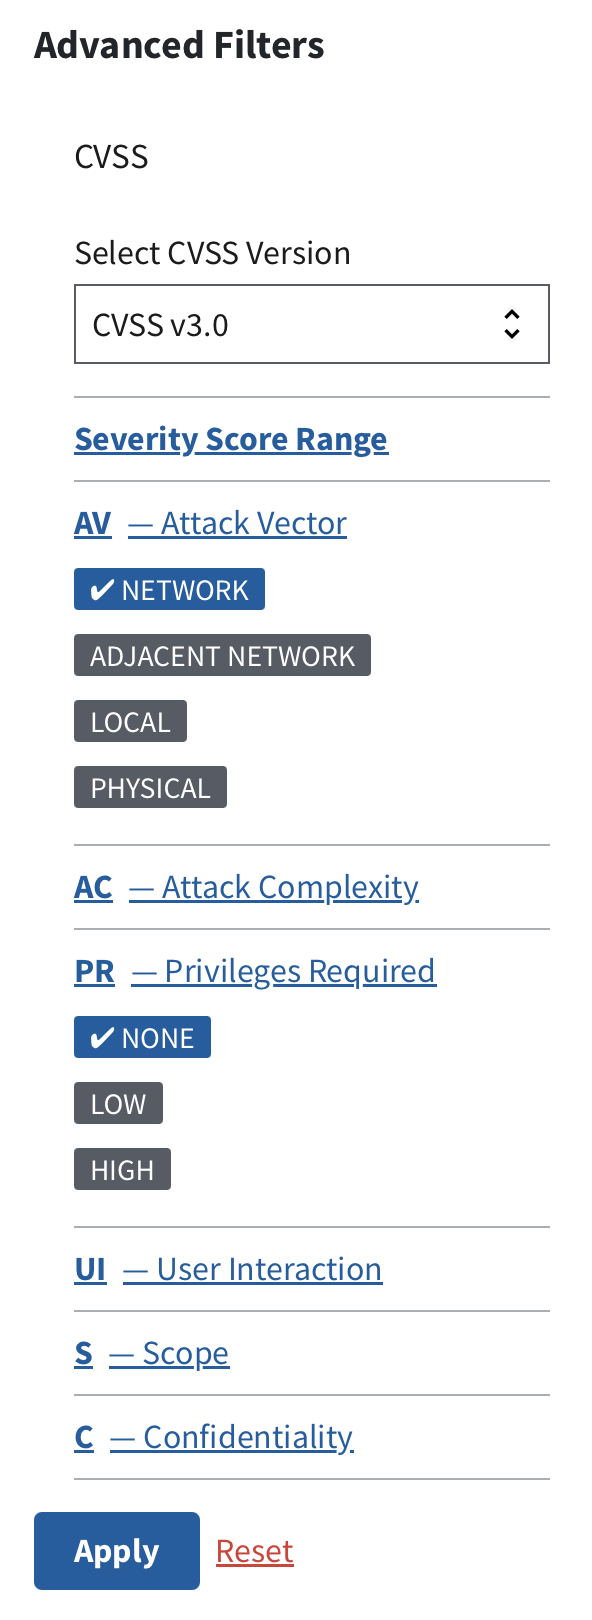
\includegraphics[width=\textwidth]{Imagenes/03-SearchFilter-1.png}
        \caption{Filtros de rango de fechas (\textit{Last Modified} y \textit{Published}).}
    \end{subfigure}
    \hfill
    \begin{subfigure}[t]{0.48\textwidth}
        \centering
        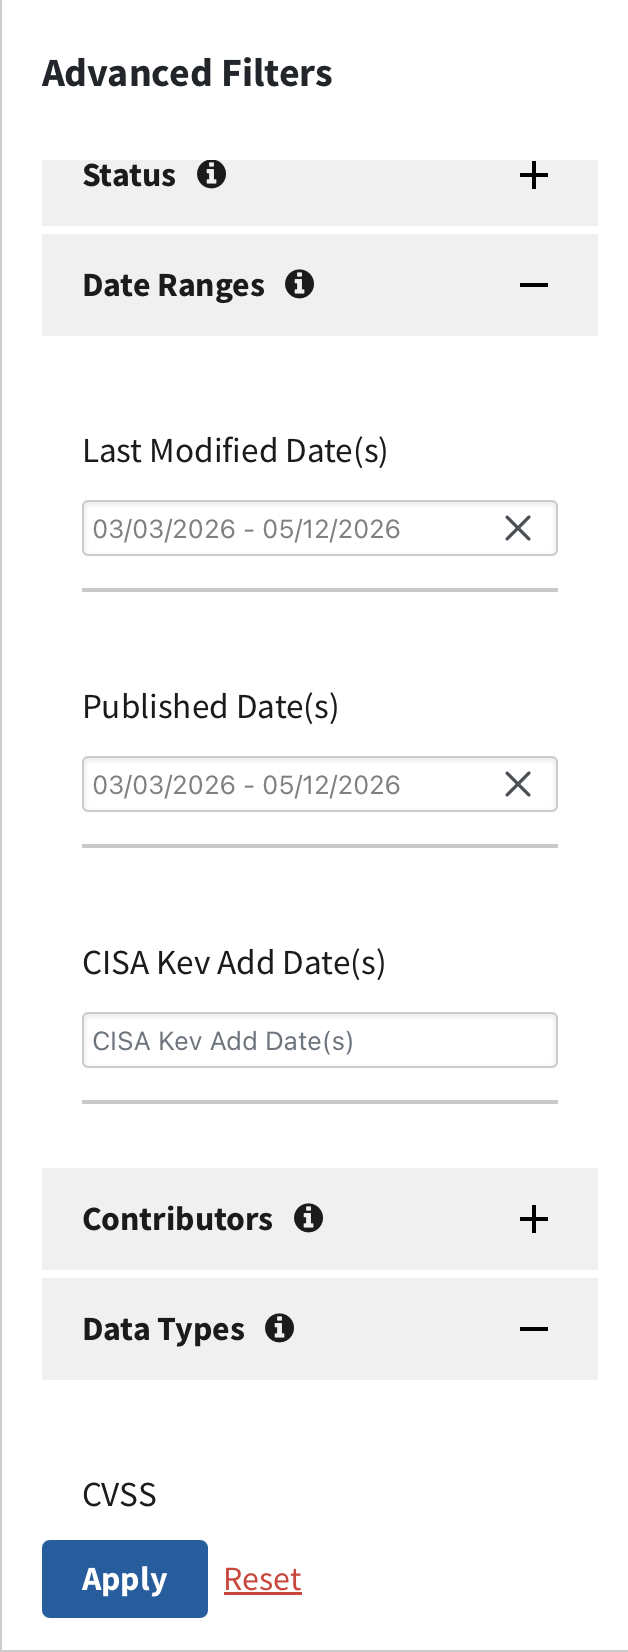
\includegraphics[width=\textwidth]{Imagenes/04-SearchFilter-2.png}
        \caption{Filtros CVSS aplicados: \texttt{AV:N} y \texttt{PR:N}.}
    \end{subfigure}
    \caption{Filtros avanzados utilizados en la búsqueda sobre la NVD.}
\end{figure}

Los filtros aplicados sobre cada ventana de tres meses fueron, de forma consistente: \textit{CVSS v3.x}, \textit{Severity = Critical}, \textit{Attack Vector = Network} y \textit{Privileges Required = None}. Sobre el listado resultante se descartaron manualmente las entradas correspondientes a aplicaciones de terceros (navegadores, suites ofimáticas, reproductores, etc.) hasta acotar el conjunto a candidatos relevantes para los criterios del enunciado.

\section{Candidatos descartados}

Durante el proceso de selección se evaluaron y descartaron varias CVE que en principio aparecían en los listados filtrados. La siguiente tabla recoge los descartes más representativos y el motivo concreto en cada caso:

\begin{table}[H]
\centering
\renewcommand{\arraystretch}{1.3}
\begin{tabularx}{\textwidth}{|l|l|X|}
\hline
\rowcolor{lightblue}
\textbf{Identificador} & \textbf{Plataforma} & \textbf{Razón del descarte} \\ \hline
CVE-2025-21298 & Windows & Vulnerabilidad crítica en Windows OLE (CVSS 9.8). Se descartó porque ya estaba cubierta la plataforma Windows por CVE-2025-53766, que afecta a un componente gráfico (GDI+) de uso más transversal y por tanto de mayor interés didáctico. \\ \hline
CVE-2025-32711 & Multiplataforma & Vulnerabilidad crítica de \textit{prompt injection} sobre Microsoft 365 Copilot (\textit{EchoLeak}, CVSS 9.3). Aunque cumple los requisitos de puntuación y vector, afecta a una aplicación SaaS de terceros, no a un componente del sistema operativo base. \\ \hline
CVE-2025-49144 & Windows & Notepad++ \textit{installer privilege escalation}. Descartada porque, pese a la alta puntuación, el componente afectado es una aplicación de terceros y el vector real requiere ejecución local del instalador, no encajando con el espíritu del criterio \texttt{AV:N}. \\ \hline
CVE-2024-43461 & Windows & Spoofing en Windows MSHTML Platform (CVSS 8.8). Se descartó por puntuación por debajo del umbral 9.0 y porque la métrica UI:R (\textit{User Interaction Required}) restaba interés frente a otros candidatos con \texttt{UI:N}. \\ \hline
\end{tabularx}
\caption{Candidatos descartados durante el proceso de selección.}
\end{table}

La elección final responde a un equilibrio entre \textit{diversidad de plataformas}, \textit{naturaleza del componente afectado} y \textit{actualidad del registro}. CVE-2025-53766 es el caso prototípico de vulnerabilidad crítica reciente en una biblioteca \textbf{nativa de Windows} (GDI+), con parche oficial dentro del ciclo \textit{Patch Tuesday}. CVE-2023-51582 cubre la plataforma \textbf{Linux} con un fallo de ejecución remota de código en un servicio que se distribuye \textit{con privilegios elevados} sobre la propia plataforma, y cuyo registro ha sido reanalizado por la NVD dentro del plazo exigido. Por último, CVE-2018-6350 aporta la perspectiva del mundo \textbf{móvil} (Android e iOS) sobre un componente \textit{de comunicaciones} (parser RTP) instalado de fábrica en la práctica totalidad de los terminales actuales, y su republicación en marzo de 2025 la sitúa también dentro de la ventana temporal de la práctica. El conjunto cubre, por tanto, tres familias de sistemas operativos representativas y tres tipos de impacto técnico distintos: corrupción de memoria en una biblioteca gráfica, exposición de un método peligroso en un servicio de red y lectura fuera de límites en un parser de protocolo.
